
\chapter{Implementation and Results}

\section{Simulation}\label{section:Implementation}
Simulation using path generation, path following control and EKF combined.
\section{Hardware}\label{section:Hardware}
Verify EKF using Hardware
Description of the Hardware
Pixhawk 2.1 CubeBlack, Intel Edison, APSync, Ardupilot ArduCopter 4.1. 
Sensors onboard the Cube, plus OFS and GPS external sensors.

In addition to the simulation results, test flights were conducted with a custom hexacopter with the aim of collecting data to verify the EKF algorithm.

\begin{figure}[htb]
	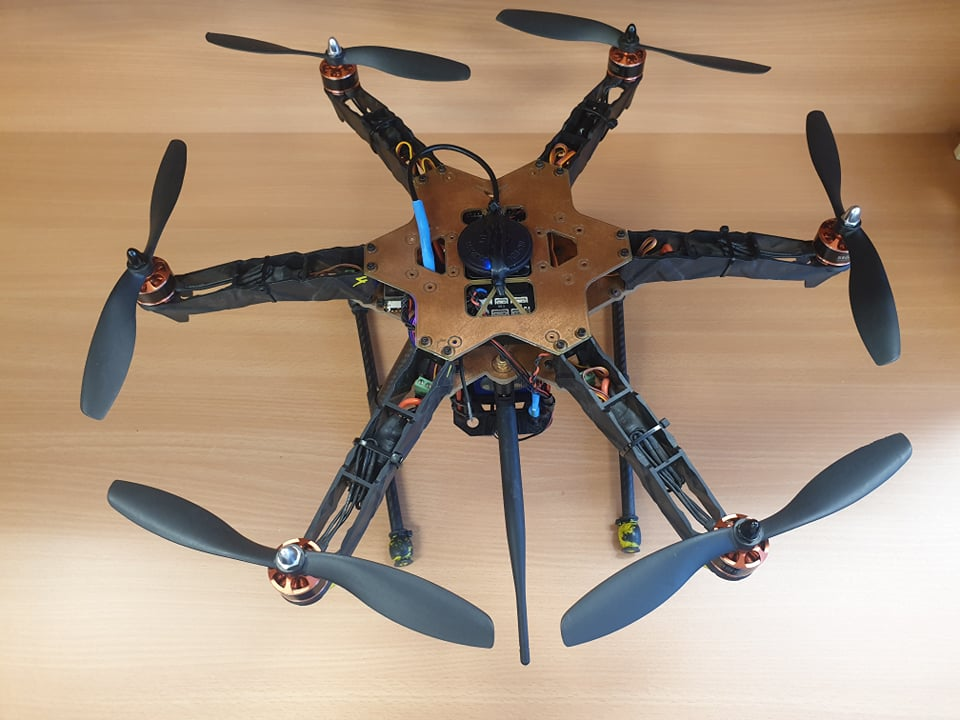
\includegraphics[width=\columnwidth]{Hexacopter_Hardware.jpg}%
	\caption{Hardware platform used for flight testing.}%
	\label{fig:hardware}%
\end{figure}

\subsection{The Cube Autopilot}
The drone is controlled by a commercial flight controller known as The Cube Autopilot (formerly known as Pixhawk 2.1).
\subsection{ArduPilot Software}
The vehicle is controlled using the open source flight software Ardupilot, with the specific version being ArduCopter 4.1.
\subsection{Companion Computer}
Additionally, a computer-on-module known as the Intel Edison was added to the Cube flight controller in order to enhance the system capabilities and enable wireless communication. The Edison has a 500 MHz dual-core processor, 1 GB RAM, 4 GB storage and dual-band (2.4 and 5 GHz) WiFi connectivity.

APSync, an open source Linux distribution developed for use with ArduPilot, was installed as the operating system on the Edison. APSync also includes python and dronekit packages preinstalled. Dronekit is an open source API which allows python scripts to be run on flight control hardware. The relationship between the different systems is shown in figure .......

\subsection{Flight Testing}
Flight testing was conducted by programming the hexacopter with an autonomous mission. The mission involved taking off to a height of 1.5 metres, travelling approximately 11 metres to a second position and then landing. The drone performed the mission successfully using the ArduPilot flight control software and the sensor data during the flight was logged to the onboard SD card. This data was then processed in MATLAB and used with the EKF algorithm described in Section \ref{section:}. The results of this EKF data are then compared with the state values estimated by the ArduPilot EKF. Figures \figref{}, \figref{} show these results.

A flight test was then repeated with the optical flow sensor installed, in order to evaluate the effectiveness of the EKF in the absence of GPS data. The results of this flight test is shown in Figures \figref{}.

\section{Chapter Summary}

\clearpage


